\documentclass{extbook}[14pt]
\usepackage{multicol, enumerate, enumitem, hyperref, color, soul, setspace, parskip, fancyhdr, amssymb, amsthm, amsmath, latexsym, units, mathtools}
\everymath{\displaystyle}
\usepackage[headsep=0.5cm,headheight=0cm, left=1 in,right= 1 in,top= 1 in,bottom= 1 in]{geometry}
\usepackage{dashrule}  % Package to use the command below to create lines between items
\newcommand{\litem}[1]{\item #1

\rule{\textwidth}{0.4pt}}
\pagestyle{fancy}
\lhead{}
\chead{Answer Key for Progress Quiz 6 Version C}
\rhead{}
\lfoot{4563-7456}
\cfoot{}
\rfoot{Summer C 2021}
\begin{document}
\textbf{This key should allow you to understand why you choose the option you did (beyond just getting a question right or wrong). \href{https://xronos.clas.ufl.edu/mac1105spring2020/courseDescriptionAndMisc/Exams/LearningFromResults}{More instructions on how to use this key can be found here}.}

\textbf{If you have a suggestion to make the keys better, \href{https://forms.gle/CZkbZmPbC9XALEE88}{please fill out the short survey here}.}

\textit{Note: This key is auto-generated and may contain issues and/or errors. The keys are reviewed after each exam to ensure grading is done accurately. If there are issues (like duplicate options), they are noted in the offline gradebook. The keys are a work-in-progress to give students as many resources to improve as possible.}

\rule{\textwidth}{0.4pt}

\begin{enumerate}\litem{
Construct the lowest-degree polynomial given the zeros below. Then, choose the intervals that contain the coefficients of the polynomial in the form $x^3+bx^2+cx+d$.
\[ -2 - 5 i \text{ and } 3 \]The solution is \( x^{3} + x^{2} +17 x -87 \), which is option A.\begin{enumerate}[label=\Alph*.]
\item \( b \in [-0.9, 3.8], c \in [16, 20.1], \text{ and } d \in [-91, -82] \)

* $x^{3} + x^{2} +17 x -87$, which is the correct option.
\item \( b \in [-1.5, 0.8], c \in [16, 20.1], \text{ and } d \in [84, 91] \)

$x^{3} -1 x^{2} +17 x + 87$, which corresponds to multiplying out $(x-(-2 - 5 i))(x-(-2 + 5 i))(x + 3)$.
\item \( b \in [-0.9, 3.8], c \in [-3.2, -0.5], \text{ and } d \in [-6, -1] \)

$x^{3} + x^{2} -x -6$, which corresponds to multiplying out $(x + 2)(x -3)$.
\item \( b \in [-0.9, 3.8], c \in [0.2, 7.4], \text{ and } d \in [-15, -11] \)

$x^{3} + x^{2} +2 x -15$, which corresponds to multiplying out $(x + 5)(x -3)$.
\item \( \text{None of the above.} \)

This corresponds to making an unanticipated error or not understanding how to use nonreal complex numbers to create the lowest-degree polynomial. If you chose this and are not sure what you did wrong, please contact the coordinator for help.
\end{enumerate}

\textbf{General Comment:} Remember that the conjugate of $a+bi$ is $a-bi$. Since these zeros always come in pairs, we need to multiply out $(x-(-2 - 5 i))(x-(-2 + 5 i))(x-(3))$.
}
\litem{
Which of the following equations \textit{could} be of the graph presented below?

\begin{center}
    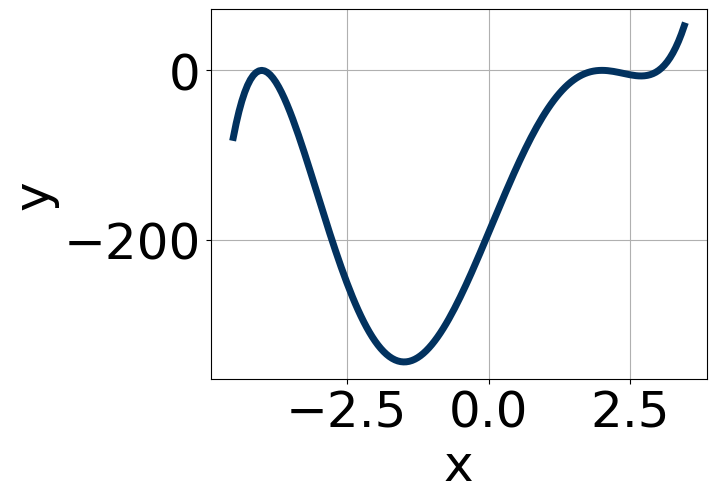
\includegraphics[width=0.5\textwidth]{../Figures/polyGraphToFunctionC.png}
\end{center}


The solution is \( 8(x + 4)^{6} (x - 2)^{8} (x - 3)^{9} \), which is option C.\begin{enumerate}[label=\Alph*.]
\item \( 13(x + 4)^{6} (x - 2)^{5} (x - 3)^{9} \)

The factor $(x - 2)$ should have an even power.
\item \( -18(x + 4)^{4} (x - 2)^{10} (x - 3)^{6} \)

The factor $(x - 3)$ should have an odd power and the leading coefficient should be the opposite sign.
\item \( 8(x + 4)^{6} (x - 2)^{8} (x - 3)^{9} \)

* This is the correct option.
\item \( 3(x + 4)^{8} (x - 2)^{9} (x - 3)^{4} \)

The factor $(x - 2)$ should have an even power and the factor $(x - 3)$ should have an odd power.
\item \( -8(x + 4)^{4} (x - 2)^{8} (x - 3)^{5} \)

This corresponds to the leading coefficient being the opposite value than it should be.
\end{enumerate}

\textbf{General Comment:} General Comments: Draw the x-axis to determine which zeros are touching (and so have even multiplicity) or cross (and have odd multiplicity).
}
\litem{
Which of the following equations \textit{could} be of the graph presented below?

\begin{center}
    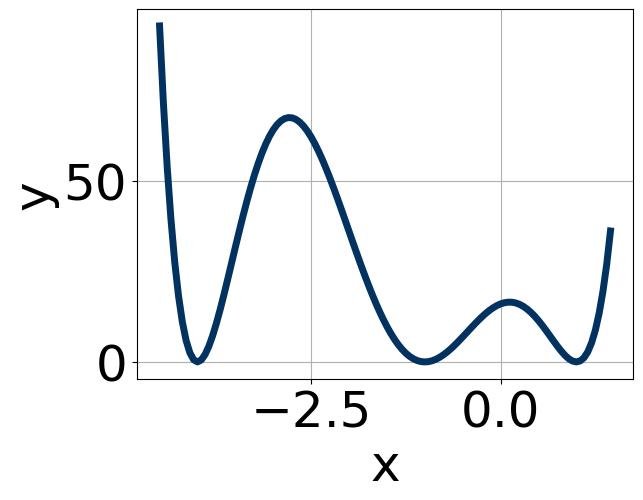
\includegraphics[width=0.5\textwidth]{../Figures/polyGraphToFunctionCopyC.png}
\end{center}


The solution is \( 18(x + 4)^{6} (x + 1)^{4} (x - 1)^{8} \), which is option C.\begin{enumerate}[label=\Alph*.]
\item \( -18(x + 4)^{10} (x + 1)^{4} (x - 1)^{8} \)

This corresponds to the leading coefficient being the opposite value than it should be.
\item \( 20(x + 4)^{8} (x + 1)^{5} (x - 1)^{7} \)

The factors $(x + 1)$ and $(x - 1)$ should both have even powers.
\item \( 18(x + 4)^{6} (x + 1)^{4} (x - 1)^{8} \)

* This is the correct option.
\item \( -4(x + 4)^{10} (x + 1)^{10} (x - 1)^{7} \)

The factor $(x - 1)$ should have an even power and the leading coefficient should be the opposite sign.
\item \( 6(x + 4)^{8} (x + 1)^{4} (x - 1)^{7} \)

The factor $(x - 1)$ should have an even power.
\end{enumerate}

\textbf{General Comment:} General Comments: Draw the x-axis to determine which zeros are touching (and so have even multiplicity) or cross (and have odd multiplicity).
}
\litem{
Describe the zero behavior of the zero $x = 6$ of the polynomial below.
\[ f(x) = -3(x + 4)^{8}(x - 4)^{5}(x + 6)^{6}(x - 6)^{5} \]The solution is the graph below, which is option A.
    \begin{center}
        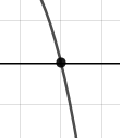
\includegraphics[width=0.3\textwidth]{../Figures/polyZeroBehaviorCopyAC.png}
    \end{center}\begin{enumerate}[label=\Alph*.]
\begin{multicols}{2}
\item 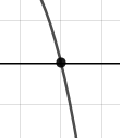
\includegraphics[width = 0.3\textwidth]{../Figures/polyZeroBehaviorCopyAC.png}
\item 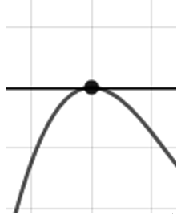
\includegraphics[width = 0.3\textwidth]{../Figures/polyZeroBehaviorCopyBC.png}
\item 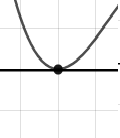
\includegraphics[width = 0.3\textwidth]{../Figures/polyZeroBehaviorCopyCC.png}
\item 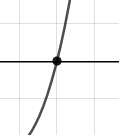
\includegraphics[width = 0.3\textwidth]{../Figures/polyZeroBehaviorCopyDC.png}
\end{multicols}\item None of the above.\end{enumerate}
\textbf{General Comment:} You will need to sketch the entire graph, then zoom in on the zero the question asks about.
}
\litem{
Construct the lowest-degree polynomial given the zeros below. Then, choose the intervals that contain the coefficients of the polynomial in the form $x^3+bx^2+cx+d$.
\[ -2 + 5 i \text{ and } 1 \]The solution is \( x^{3} +3 x^{2} +25 x -29 \), which is option A.\begin{enumerate}[label=\Alph*.]
\item \( b \in [2.3, 3.6], c \in [24, 32], \text{ and } d \in [-30, -20] \)

* $x^{3} +3 x^{2} +25 x -29$, which is the correct option.
\item \( b \in [-1.2, 1.7], c \in [-10, -3], \text{ and } d \in [0, 12] \)

$x^{3} + x^{2} -6 x + 5$, which corresponds to multiplying out $(x -5)(x -1)$.
\item \( b \in [-1.2, 1.7], c \in [-1, 13], \text{ and } d \in [-5, 0] \)

$x^{3} + x^{2} +x -2$, which corresponds to multiplying out $(x + 2)(x -1)$.
\item \( b \in [-5.5, -1.7], c \in [24, 32], \text{ and } d \in [23, 32] \)

$x^{3} -3 x^{2} +25 x + 29$, which corresponds to multiplying out $(x-(-2 + 5 i))(x-(-2 - 5 i))(x + 1)$.
\item \( \text{None of the above.} \)

This corresponds to making an unanticipated error or not understanding how to use nonreal complex numbers to create the lowest-degree polynomial. If you chose this and are not sure what you did wrong, please contact the coordinator for help.
\end{enumerate}

\textbf{General Comment:} Remember that the conjugate of $a+bi$ is $a-bi$. Since these zeros always come in pairs, we need to multiply out $(x-(-2 + 5 i))(x-(-2 - 5 i))(x-(1))$.
}
\litem{
Construct the lowest-degree polynomial given the zeros below. Then, choose the intervals that contain the coefficients of the polynomial in the form $ax^3+bx^2+cx+d$.
\[ 2, \frac{1}{5}, \text{ and } \frac{-1}{4} \]The solution is \( 20x^{3} -39 x^{2} -3 x + 2 \), which is option C.\begin{enumerate}[label=\Alph*.]
\item \( a \in [17, 29], b \in [-39.3, -36.6], c \in [-5.1, -0.4], \text{ and } d \in [-4, 0] \)

$20x^{3} -39 x^{2} -3 x -2$, which corresponds to multiplying everything correctly except the constant term.
\item \( a \in [17, 29], b \in [47.6, 51.5], c \in [18.7, 20.3], \text{ and } d \in [2, 8] \)

$20x^{3} +49 x^{2} +19 x + 2$, which corresponds to multiplying out $(x + 2)(5x + 1)(4x + 1)$.
\item \( a \in [17, 29], b \in [-39.3, -36.6], c \in [-5.1, -0.4], \text{ and } d \in [2, 8] \)

* $20x^{3} -39 x^{2} -3 x + 2$, which is the correct option.
\item \( a \in [17, 29], b \in [33.4, 40.5], c \in [-5.1, -0.4], \text{ and } d \in [-4, 0] \)

$20x^{3} +39 x^{2} -3 x -2$, which corresponds to multiplying out $(x + 2)(5x + 1)(4x -1)$.
\item \( a \in [17, 29], b \in [39.7, 41.9], c \in [-2, 2.2], \text{ and } d \in [-4, 0] \)

$20x^{3} +41 x^{2} +x -2$, which corresponds to multiplying out $(x + 2)(5x -1)(4x + 1)$.
\end{enumerate}

\textbf{General Comment:} To construct the lowest-degree polynomial, you want to multiply out $(x -2)(5x -1)(4x + 1)$
}
\litem{
Describe the end behavior of the polynomial below.
\[ f(x) = 5(x - 5)^{4}(x + 5)^{5}(x - 6)^{5}(x + 6)^{6} \]The solution is the graph below, which is option C.
    \begin{center}
        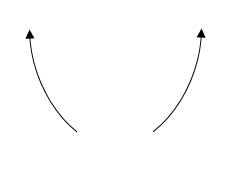
\includegraphics[width=0.3\textwidth]{../Figures/polyEndBehaviorCC.png}
    \end{center}\begin{enumerate}[label=\Alph*.]
\begin{multicols}{2}
\item 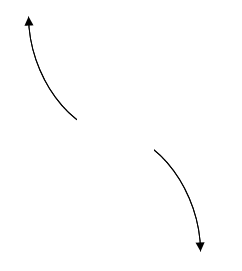
\includegraphics[width = 0.3\textwidth]{../Figures/polyEndBehaviorAC.png}
\item 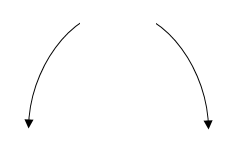
\includegraphics[width = 0.3\textwidth]{../Figures/polyEndBehaviorBC.png}
\item 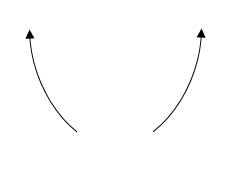
\includegraphics[width = 0.3\textwidth]{../Figures/polyEndBehaviorCC.png}
\item 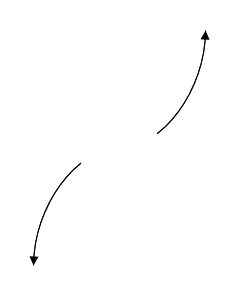
\includegraphics[width = 0.3\textwidth]{../Figures/polyEndBehaviorDC.png}
\end{multicols}\item None of the above.\end{enumerate}
\textbf{General Comment:} Remember that end behavior is determined by the leading coefficient AND whether the \textbf{sum} of the multiplicities is positive or negative.
}
\litem{
Construct the lowest-degree polynomial given the zeros below. Then, choose the intervals that contain the coefficients of the polynomial in the form $ax^3+bx^2+cx+d$.
\[ -5, \frac{-2}{3}, \text{ and } \frac{-7}{5} \]The solution is \( 15x^{3} +106 x^{2} +169 x + 70 \), which is option E.\begin{enumerate}[label=\Alph*.]
\item \( a \in [12, 16], b \in [103, 110], c \in [161, 178], \text{ and } d \in [-74, -62] \)

$15x^{3} +106 x^{2} +169 x -70$, which corresponds to multiplying everything correctly except the constant term.
\item \( a \in [12, 16], b \in [-72, -57], c \in [-75, -65], \text{ and } d \in [68, 74] \)

$15x^{3} -64 x^{2} -69 x + 70$, which corresponds to multiplying out $(x -5)(3x -2)(5x + 7)$.
\item \( a \in [12, 16], b \in [-45, -43], c \in [-142, -136], \text{ and } d \in [-74, -62] \)

$15x^{3} -44 x^{2} -141 x -70$, which corresponds to multiplying out $(x -5)(3x + 2)(5x + 7)$.
\item \( a \in [12, 16], b \in [-113, -105], c \in [161, 178], \text{ and } d \in [-74, -62] \)

$15x^{3} -106 x^{2} +169 x -70$, which corresponds to multiplying out $(x -5)(3x -2)(5x -7)$.
\item \( a \in [12, 16], b \in [103, 110], c \in [161, 178], \text{ and } d \in [68, 74] \)

* $15x^{3} +106 x^{2} +169 x + 70$, which is the correct option.
\end{enumerate}

\textbf{General Comment:} To construct the lowest-degree polynomial, you want to multiply out $(x + 5)(3x + 2)(5x + 7)$
}
\litem{
Describe the zero behavior of the zero $x = -9$ of the polynomial below.
\[ f(x) = -9(x - 9)^{4}(x + 9)^{5}(x + 3)^{9}(x - 3)^{10} \]The solution is the graph below, which is option D.
    \begin{center}
        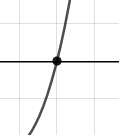
\includegraphics[width=0.3\textwidth]{../Figures/polyZeroBehaviorDC.png}
    \end{center}\begin{enumerate}[label=\Alph*.]
\begin{multicols}{2}
\item 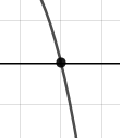
\includegraphics[width = 0.3\textwidth]{../Figures/polyZeroBehaviorAC.png}
\item 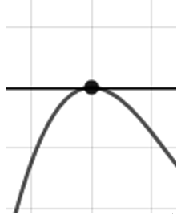
\includegraphics[width = 0.3\textwidth]{../Figures/polyZeroBehaviorBC.png}
\item 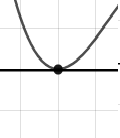
\includegraphics[width = 0.3\textwidth]{../Figures/polyZeroBehaviorCC.png}
\item 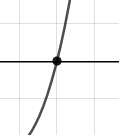
\includegraphics[width = 0.3\textwidth]{../Figures/polyZeroBehaviorDC.png}
\end{multicols}\item None of the above.\end{enumerate}
\textbf{General Comment:} You will need to sketch the entire graph, then zoom in on the zero the question asks about.
}
\litem{
Describe the end behavior of the polynomial below.
\[ f(x) = 5(x - 5)^{5}(x + 5)^{10}(x - 8)^{5}(x + 8)^{7} \]The solution is the graph below, which is option D.
    \begin{center}
        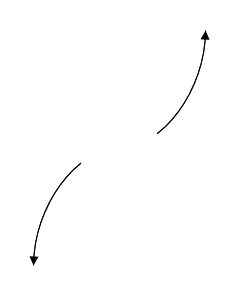
\includegraphics[width=0.3\textwidth]{../Figures/polyEndBehaviorCopyDC.png}
    \end{center}\begin{enumerate}[label=\Alph*.]
\begin{multicols}{2}
\item 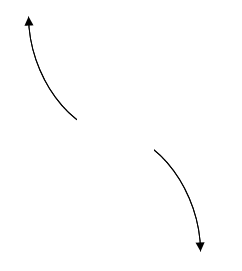
\includegraphics[width = 0.3\textwidth]{../Figures/polyEndBehaviorCopyAC.png}
\item 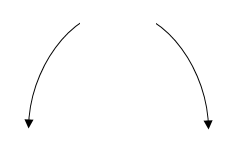
\includegraphics[width = 0.3\textwidth]{../Figures/polyEndBehaviorCopyBC.png}
\item 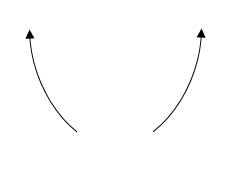
\includegraphics[width = 0.3\textwidth]{../Figures/polyEndBehaviorCopyCC.png}
\item 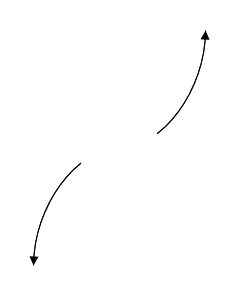
\includegraphics[width = 0.3\textwidth]{../Figures/polyEndBehaviorCopyDC.png}
\end{multicols}\item None of the above.\end{enumerate}
\textbf{General Comment:} Remember that end behavior is determined by the leading coefficient AND whether the \textbf{sum} of the multiplicities is positive or negative.
}
\end{enumerate}

\end{document}